%!TEX root = ClementiBarba2020.tex

These first set of results correspond to the replication study of some results 
of Rockstuhl et al, 2005 \cite{rockstuhl2005}. Rockstuhl and coworkers did a two dimension 
study of the phonon-polariton response of different nanoparticles of silicon carbide (SiC)
using a 2D boundary element method. Their limit their study to 2D shapes and assumed an infinite
third dimension. (They solved full maxwell in 2D)


We count with a 3D surface boundary element method solver, that uses the electrostatic approximation
($\lambda > d$ where $d$ is the characteristic length of the geometry). 

{\color{red}We initially produced the meshes with trimesh (not sure how to cite), later we stick to 
our own script}

Initially we attempted to perform a convergence study on the result of Figure 18a
of Rockstuhl and coworkers. This simulation consists on a "quadratic cylinder" (square)
of size $L=535$. We tried to perform convergence on a cube of the same size L, but
due to the due to the sharp edges of the geometry we were not able to see proper convergence. 
However, we did a grid independence study. We were able to show that going from a mesh of 15552 
triangles (density = 1.11x10$^-4$ $N/\text{\AA}$) to 19200 (density = 9.05x10$^-5$ $N/\text{\AA}$) 
triangles the simulations did not change at all (see Figure \ref{fig:cube535}).  

\begin{figure}
    \centering
    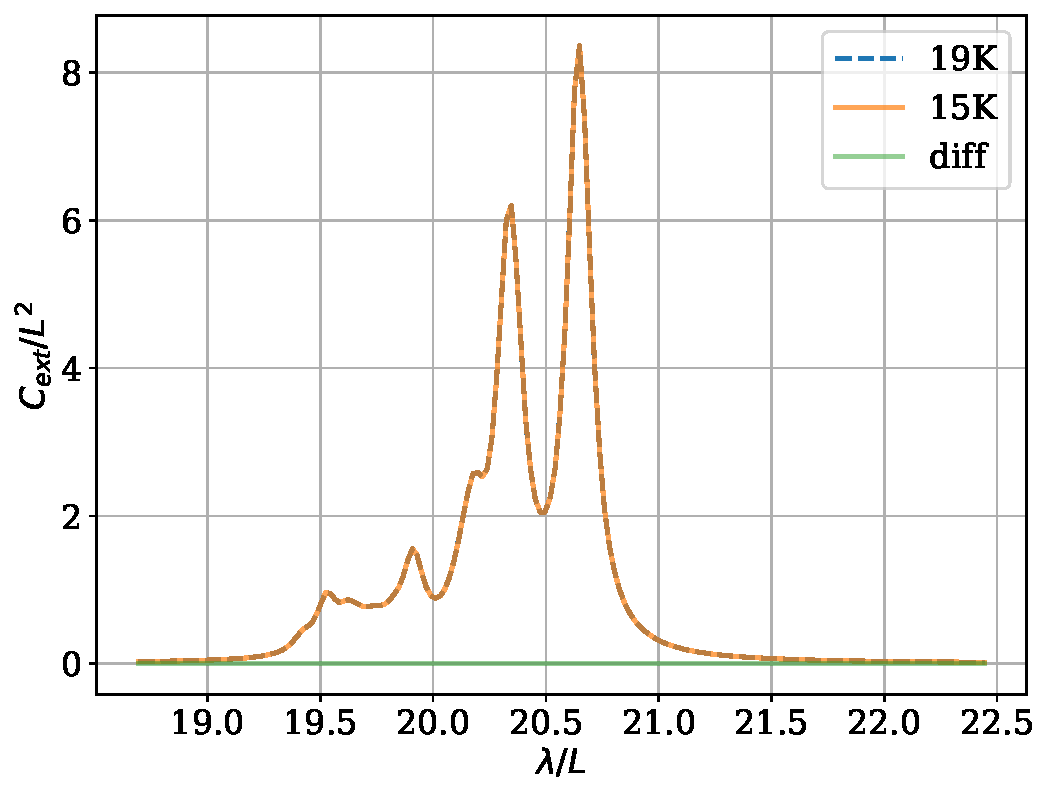
\includegraphics[width=0.85\textwidth]{cubeL535nm_15Kvs19K.pdf} 
    \caption{Extinction cross section divided by $L^2$ as a function fo wavelength divided by $L$ of
    a cube of size L=535 nm}
    \label{fig:cube535}
 \end{figure}

In this results we see extra peaks that we believe is due to the nature of our 3D model, in this case 
we have not extended the third dimension to approximate "infinity", but we suspect the extra peaks are 
due to sharpness of the edges (they mention this on their paper too) as well as the 3D nature of our solver.

These figure doesn't have the results digitized from the paper, but if needed we can add them. 

Based on these results we used the density of the cube as a reference to produce the meshes for the replication 
of figures 14a and 14b on Rockstuhl's work (case a1=672, b=328). This simulation is a "rectangular cylinder" of 
dimensions (we chose a case that will go well with our quasistatic model) are $a=672$ nm and $b=328$ nm. 

Effect of extended third dimension (in our case this is the y axis) are in Figures \ref{fig:ext_y_14a} and
\ref{fig:ext_y_14b}

\begin{figure}
    \centering
    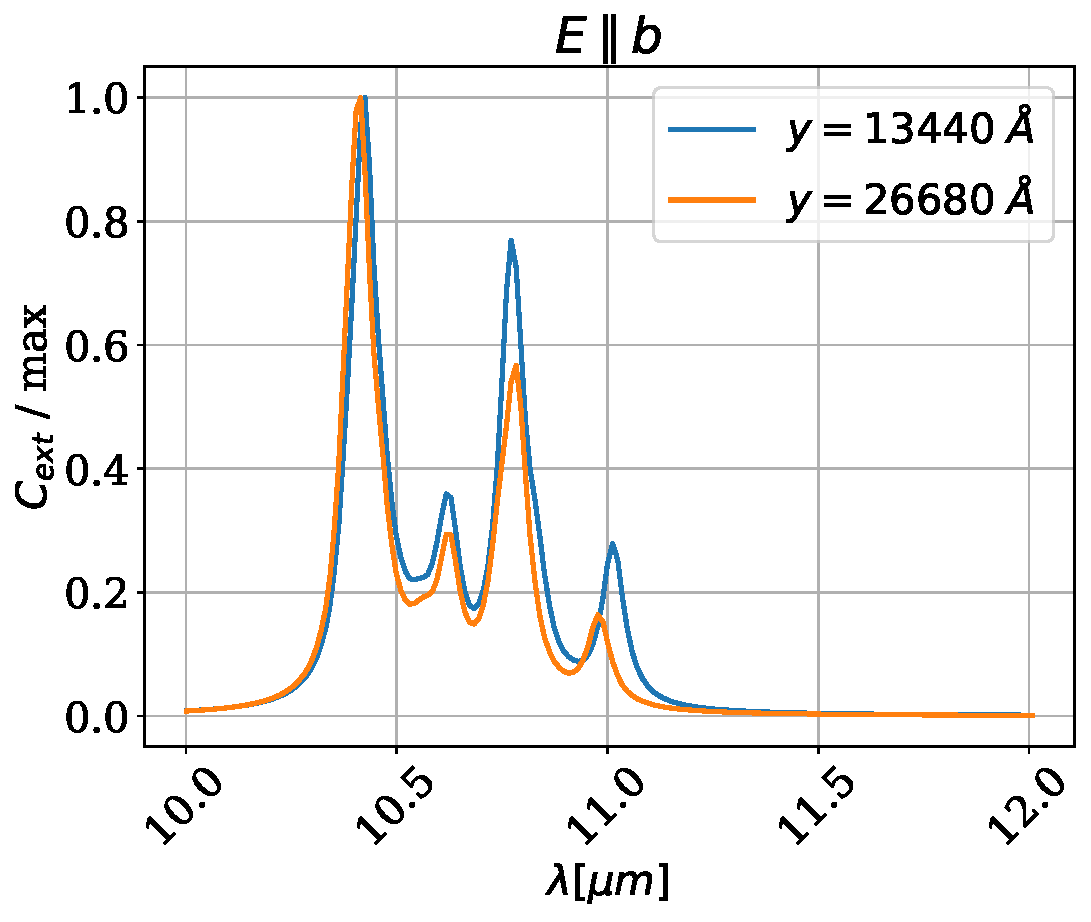
\includegraphics[width=0.85\textwidth]{ext_y_14a.pdf} 
    \caption{Normalized (by max) Extinction cross section of a rectangle for two different y-values in the 
    short edge configuration (electric field parallel to the shorter dimension)}
    \label{fig:ext_y_14a}
 \end{figure}

 \begin{figure}
    \centering
    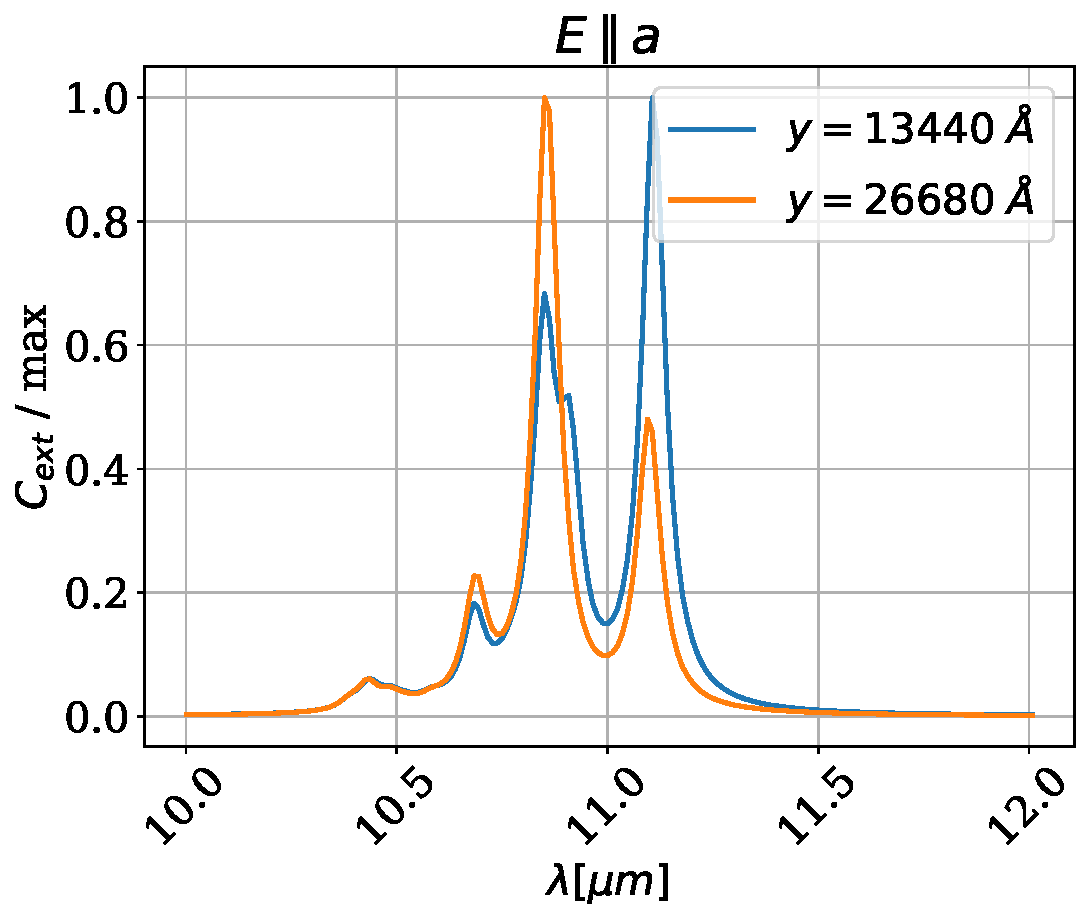
\includegraphics[width=0.85\textwidth]{ext_y_14b.pdf} 
    \caption{Normalized (by max) Extinction cross section of a rectangle for two different y-values in the 
    long edge configuration (electric field parallel to the longer dimension)}
    \label{fig:ext_y_14b}
 \end{figure}

We see that as we elongate the third dimension the extra peaks start fading. 

At this point we noticed that the mesher (trimesh) was not generating a uniform mesh. We created our 
own mesher, and tested the difference. Moreover, the paper mentioned that they rounded the corners of their
"rectangular cylinder". We were able to give our mesh as input to trimesh and round the edges but we were not able 
to know how the roundness was related to the arc of the curvature. This were parameters with no physical meaning, 
therefore we decided to go with the default setting. 


\begin{figure}
    \centering
    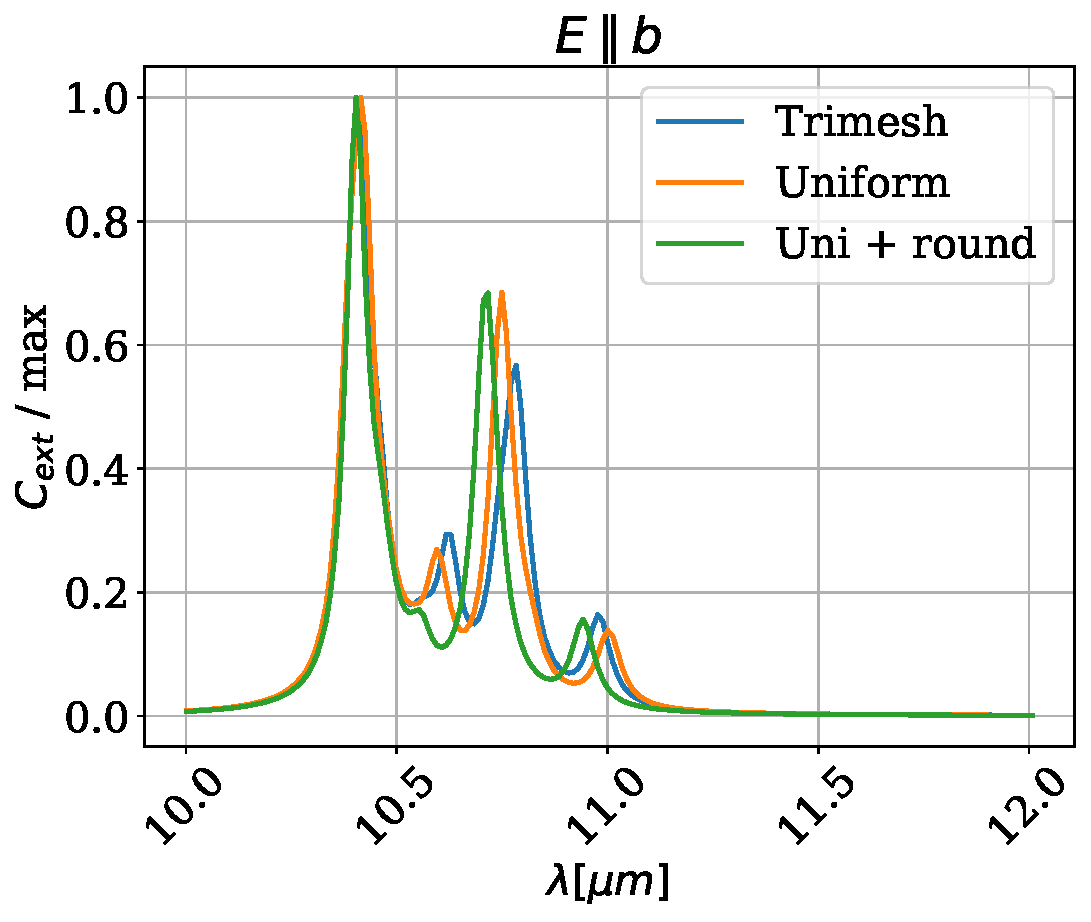
\includegraphics[width=0.85\textwidth]{tri_reg_round_14a.pdf} 
    \caption{Normalized (by max) Extinction cross section of a rectangle. Original trimesh, regular, and regular with 
    roundness. Short edge configuration (electric field parallel to the shorter dimension)}
    \label{fig:tri_reg_round_14a}
 \end{figure}

 \begin{figure}
    \centering
    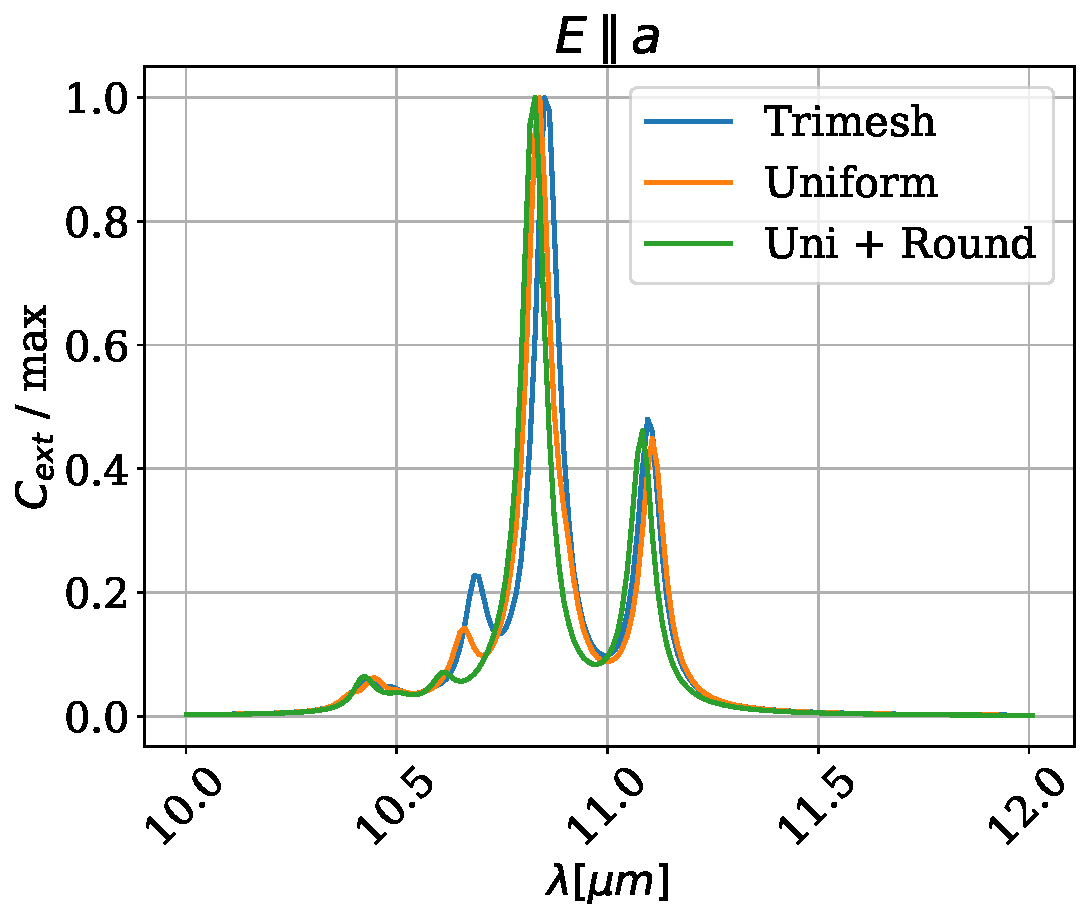
\includegraphics[width=0.85\textwidth]{tri_reg_round_14b.pdf} 
    \caption{Normalized (by max) Extinction cross section of a rectangle.  Original trimesh, regular, and regular with 
    roundness. Long edge configuration (electric field parallel to the longer dimension)}
    \label{fig:tri_reg_round_14b}
 \end{figure}


 Finally with all this info, here is the replication of Figures 14a and 14b. 

 \begin{figure}
    \centering
    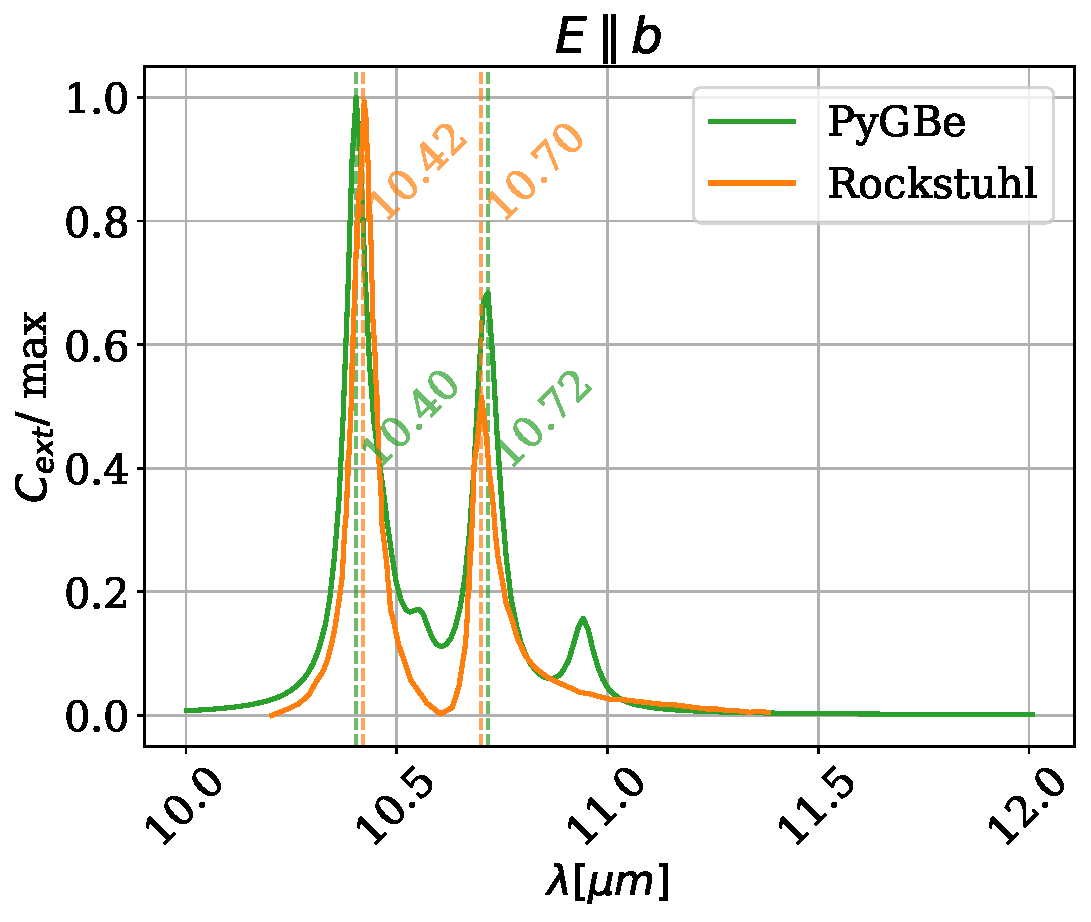
\includegraphics[width=0.85\textwidth]{replication_14a.pdf} 
    \caption{Normalized (by max) Extinction cross section of a rectangle. Replication of 
    the short edge configuration (electric field parallel to the shorter dimension)}
    \label{fig:rep_14a}
 \end{figure}

 \begin{figure}
    \centering
    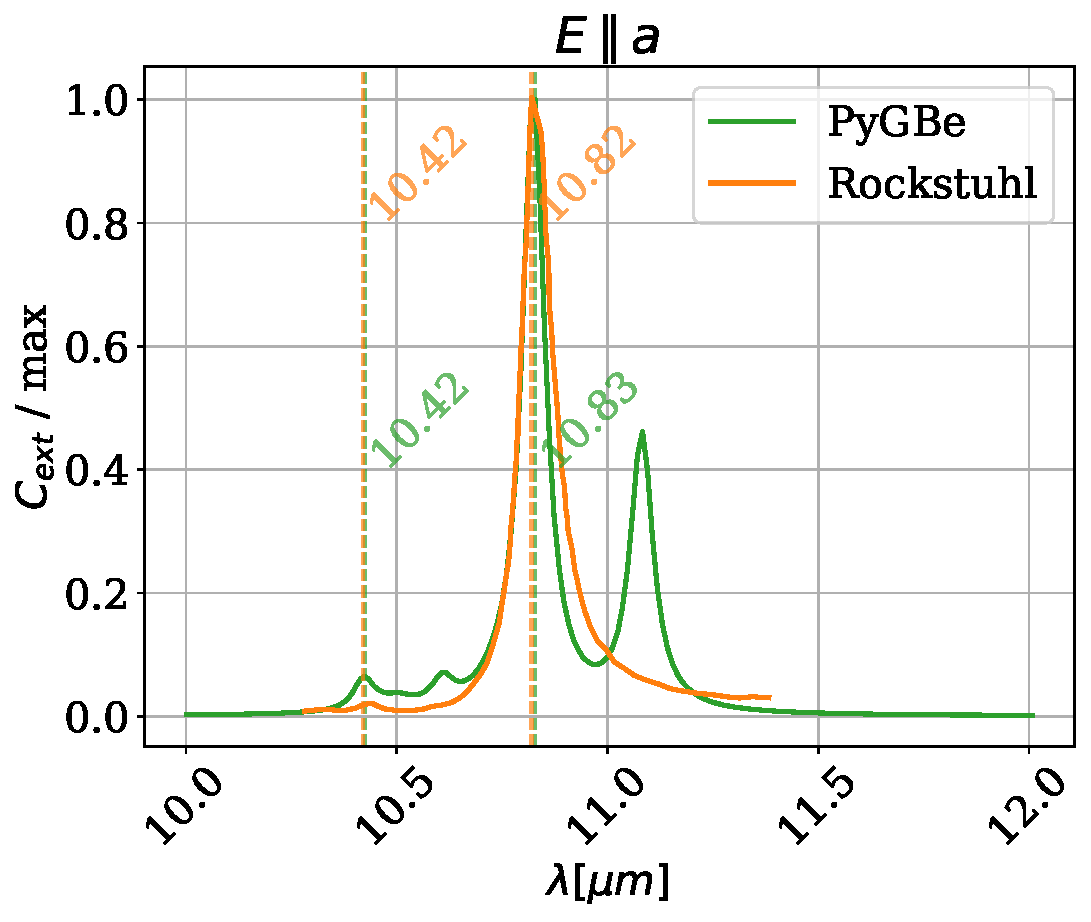
\includegraphics[width=0.85\textwidth]{replication_14b.pdf} 
    \caption{Normalized (by max) Extinction cross section of a rectangle. Replication of the 
    long edge configuration (electric field parallel to the longer dimension)}
    \label{fig:rep_14b}
 \end{figure}
